\documentclass{beamer}
\usetheme{default}

\usepackage[italian]{babel}
\usepackage[utf8x]{inputenc}

\title{Il percorso di una proposta dall'idea all'approvazione in programma, nel Partito~Pirata~Italiano}
\author{Giuseppe Cal.}
\institute{Partito Pirata Italiano -- Pirate Party of Italy}
\date{\today}

\begin{document}

\begin{frame}
\maketitle
\end{frame}

\begin{frame}{Sezioni ed aree}
LiquidFeedback 2.x divide il flusso decisionale in sezioni (\emph{units}) ed aree: 
\begin{columns}
\begin{column}{0.5\textwidth}
\begin{itemize}
\item Una \emph{sezione} raggruppa insieme aree affini, come ad esempio, quelle relative all'amministrazione piuttosto che ai contenuti o alla produzione documentale.
\item Un'\emph{area} \`e un insieme pi\`u ristretto, utile a trattare in modo diverso gli affari esteri e la regolamentazione dei trasporti, nell'esempio.
\end{itemize}
\end{column}
\begin{column}{0.5\textwidth}
\begin{figure}
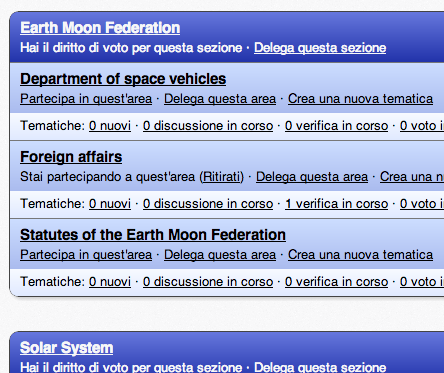
\includegraphics[width=0.95\textwidth]{pics/unitarea}
\caption{Le sezioni sulla federazione terra luna con le rispettive aree. Intravista, la sezione sul sistema solare.}
\end{figure}
\end{column}
\end{columns}
\end{frame}

\begin{frame}{Aree, ``interesse'' e quorum}
Per evitare che vengano discusse proposte poco interessanti, \`e richiesto che un certo numero di supporters portino avanti le proposte che ritengono interessanti.

Questo numero \`e regolabile per ogni area ed \`e proporzionale al numero di utenti che dicono---cliccando sull'apposito \emph{partecipa in quest'area}---di essere interessati ad un'area.
\begin{figure}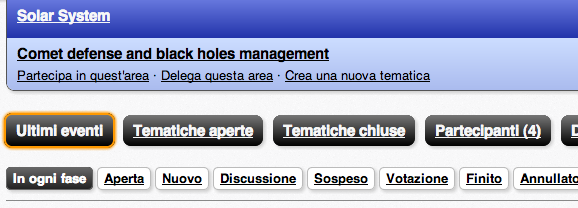
\includegraphics[width=0.8\textwidth]{pics/partecipa}
\caption{Come esprimere la propria ``partecipazione.''}
\end{figure}
\end{frame}

\begin{frame}{Aree e deleghe}
In alternativa alla partecipazione diretta, \`e possibile impostare un fiduciario che agir\`a in proprio nome all'interno di quell'area; o decidere di ignorarla del tutto, fidandosi di ci\`o che gli altri decidono. Di default, un'area eredita le impostazioni di delega della sezione che la contiene, ma \`e possibile scegliere in maniera granulare.
\begin{figure}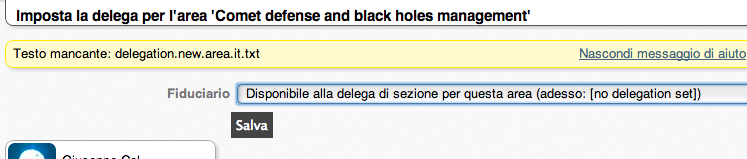
\includegraphics[width=0.8\textwidth]{pics/delega}
\caption{Deleghi qualcuno scegliendo fra i tuoi contatti e salvando.}
\end{figure}
\end{frame}

\begin{frame}{Seguire le aree}

Una volta scelte le aree che vogliamo seguire, torniamo alla home page. Da qui, cliccando su ``ultimi eventi'' possiamo vedere cosa succede nelle nostre aree preferite, ed anche in tutte le altre, giocando opportunamente con i filtri.
\begin{figure}
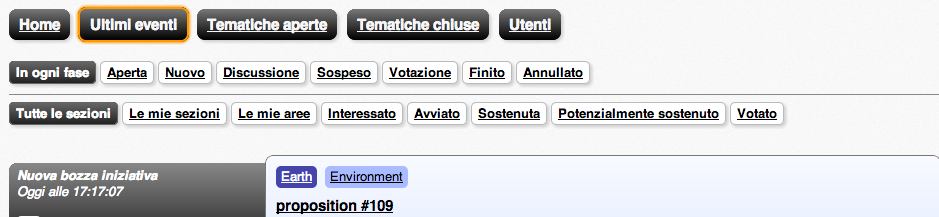
\includegraphics[width=0.99\textwidth]{pics/timeline-filters}
\caption{In alto, i filtri per scegliere cosa visualizzare. In basso, gli eventi dell'area.}
\end{figure}
\end{frame}

\begin{frame}{Creare una nuova proposta... }
\end{frame}

\begin{frame}{...o rispondere ad una gi\`a presente}
\end{frame}

\begin{frame}{Discutere con i pirati}
\end{frame}

\begin{frame}{Votare}
\end{frame}

\begin{frame}{Verificare i risultati}
\end{frame}

\end{document}
